%%%%%%%%%%%%%%%%%%%%%%%%%%%%%%%%%%%%%
%%%%% PHYS305 Assignment 5
%%%%% Zachary Martin
%%%%% 20 February 2019
%%%%%%%%%%%%%%%%%%%%%%%%%%%%%%%%%%%%%

\documentclass[aps,prl,twocolumn,superscriptaddress]{revtex4-1}

\usepackage{graphicx}  % this is the up-to-date package for all figures
\graphicspath{{pictures/}} 	% Set Graphics Path
\usepackage{siunitx} % Scientific Notation and Units
\usepackage{amsmath, amssymb, gensymb, mathtools, bm, bigints} 	% Mathematical Tools
\usepackage{verbatim}  % for the comment environment
\usepackage{color}
% \usepackage{arydshln} % Dashed lines in table

% For inserting code snippets
\usepackage{listings}
\usepackage{xcolor}
\lstset { %
    language=C++,
    backgroundcolor=\color{black!5}, % set backgroundcolor
    basicstyle=\footnotesize,% basic font setting
}

% Shortcut Commands
\newcommand{\paren}[1]{\left( #1 \right)} 	% Parentheses for complicated expressions
\newcommand{\bparen}[1]{\left[ #1 \right]}	% Bracket parentheses for complicated expressions
\newcommand{\cmod}[1]{\left| #1 \right|}	% Mod or Absolute value

\bibliographystyle{apsrev}

% these are some custom control of the page size and margins
% \topmargin= 0.2in  % these 1st two may be needed for some computers
\textheight=9in
\textwidth=6.5in
% these next two lines give us centered text
\oddsidemargin=0cm
\evensidemargin=0cm

\begin{document}

% Title Contents
\title{PHYS 305 Assignment 5: Determining the Volume of N-dimensional Spheres via Monte Carlo Integration.}
\author{Zachary Martin}
\affiliation{University of Hawaii at Manoa}
\date{20 February 2019}

\begin{abstract}
In this assignment, we introduce the use of Monte Carlo integration to examine the volume of n-dimensional hyperspheres using a program in C++. We find the odd fact that the volume of the hypersphere reaches a peak value at dimension 5 and then decreases towards 0 thereafter. We also compare the fractional error of the calculated volumes to the dimension and find that there is a fairly constant value until dimension 8, but don't have any ideas as to why this is. It is evident that a very large number of trials must be used to get decent precision and that the random nature of this method can cause fluctuations in the error when attempting to achieve high precision. 
\end{abstract}

\maketitle

\section{Introduction and Overview}

While we live spatially in three dimensions, there are times where we want to integrate over more than three dimensions to solve things about a physical system, such as 6-dimensional phase space integrals over space and momentum \citep{Laulima}. It is important then that we learn methods to integrate over these higher dimensions. While some integrals can be straight forward and have analytic solutions, this is not always the case. One way to get around this is to use Monte Carlo methods. 

The main idea of Monte Carlo integration is that we can take advantage of volume ratios of two objects, where one object contains the other (integration is equivalent to an n-dimensional volume of some function). We choose the container such that we can easily obtain the volume, such as a (hyper)cube. Then we select random points in that cube and determine whether the point is within the boundary of interest, ie. within the volume of the contained object. If we have an infinite amount of points that are truly random, then the ratio of the number of points inside the contained volume to the total number of points should be equal to ratio of the volumes. This is discussed further in the Relevant Equations section.

To demonstrate this, we begin with a simple, easy to visualize example.

\subsection{Simple Case Dim = 2, 3}

We learned how to implement randomness into a simulation using the random() function in assignment 4 \cite{rand}. Thus we can generate random points in a square of side length 2 (containing a circle of unit radius) or a cube of side length 2 (containing a sphere of unit radius) and determine the ratio of points within a radius to the total. A simulation of this Monte Carlo integration can be visualized in Figures \ref{gr:2d} and \ref{gr:3d}.

Clearly, a different number of points or trials will result in different ratios, and hence different calculated areas and volumes. We can see how the true volume compares to the calculated volume for different number of trials in Figure \ref{gr:3derr}. We can see clear fluctuations in the fractional error at low and even intermediate values of trials. This is due to the fact that it is probable that the ratio could be close to one, given the vast majority of points happen to be within a unit radius. And so we would get a ratio that implies the volume of the sphere is approximately equal to the volume of the cube. We can see it takes until at least 10000 trials to get a fairly stable value. 

\begin{figure}[htbp]
  	\begin{center}
 		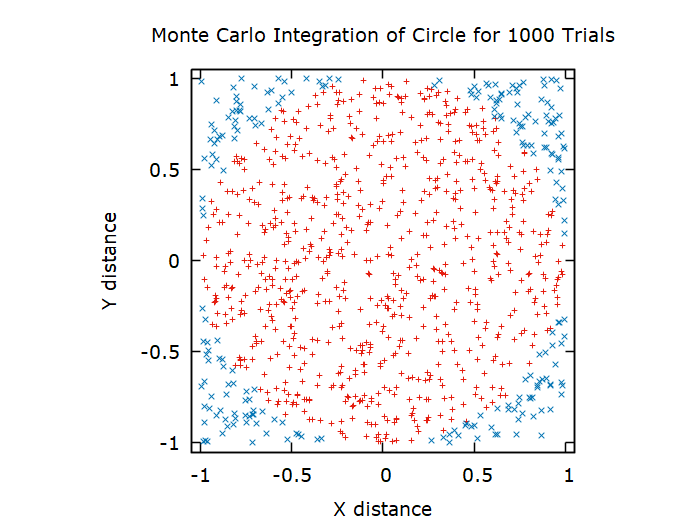
\includegraphics[scale=0.33]{pond2.png}
  		\caption{2D Case: A simulation of random points chosen within the 2x2 square. The red marks indicate a point within unit radius.}
  		\label{gr:2d}
 	\end{center}
\end{figure}

\begin{figure}[htbp]
  	\begin{center}
 		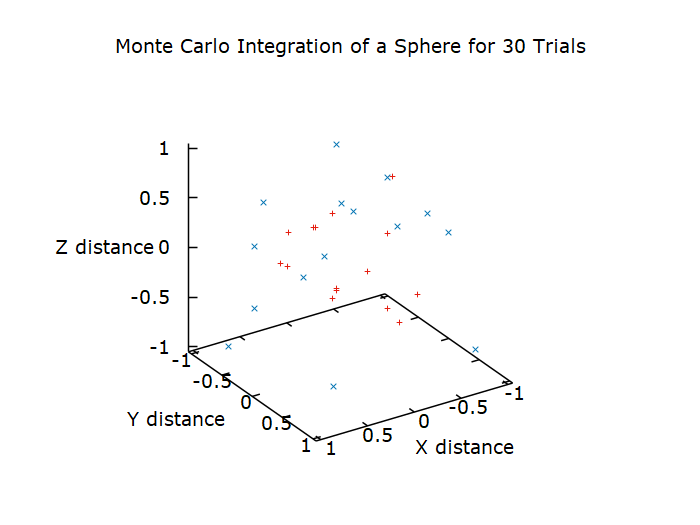
\includegraphics[scale=0.32]{30.png} 
 		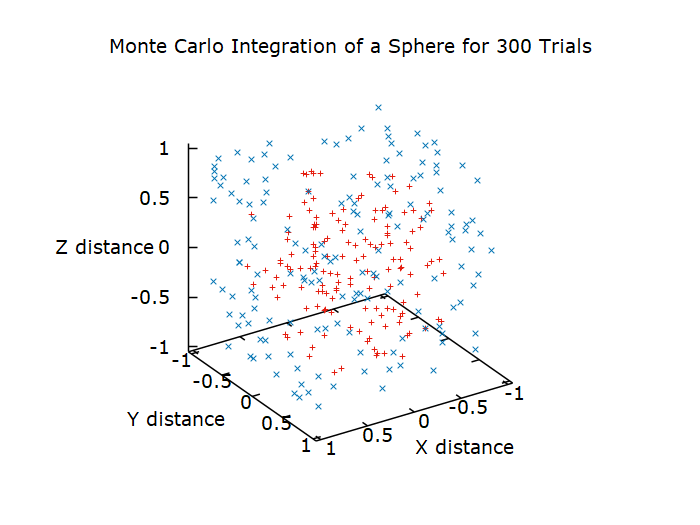
\includegraphics[scale=0.32]{300.png}
 		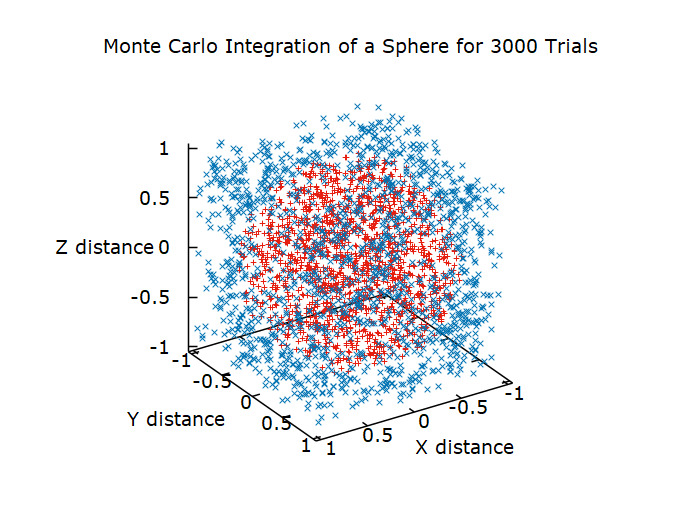
\includegraphics[scale=0.32]{3000.png}
  		\caption{3D Case: Progression of Monte Carlo simulation for 30, 300, and 3000 trials. Like with the 2D case, the red marks indicate a point within unit radius.}
  		\label{gr:3d}
 	\end{center}
\end{figure}

\begin{figure}[htbp]
  	\begin{center}
 		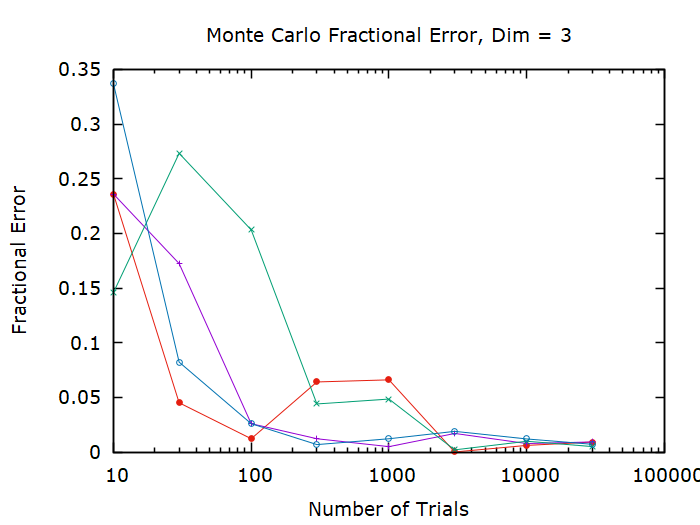
\includegraphics[scale=0.3]{pond2err.png}
  		\caption{Fractional error of the integrated volume of the unit sphere for varying numbers of trials. Each curve represents a different random seed used for generating the points inside the cube.}
  		\label{gr:3derr}
 	\end{center}
\end{figure}

Familiar with the technique, we now generalize this to $n$ dimensions.

\section{Relevant Equations}
Monte Carlo integration takes advantage of the ratio, $\alpha$, of volumes of two objects where one object contains the other. Knowing the volume of the container, $V_{\text{tot}}$, we can get \cite{Laulima}
\begin{equation}
V = \alpha V_{\text{tot}}~. \label{eqn:MC}
\end{equation}
This method finds the ratio by choosing random points within the total volume and so we can get
\begin{equation}
\alpha = \frac{N_{\text{hit}}}{N_{\text{tot}}} ~, \label{eqn:ratio}
\end{equation}
where $N_{\text{hit}}$ is the number of points within the volume of interest and $N_{\text{tot}}$ is the total number of random points within the container.
For calculating the volumes of hyperspheres, we contain the spheres within hypercubes, which have volume
\begin{equation}
V^{(n)}_{\text{cube}} = l^n ~, \label{eqn:cube}
\end{equation}
where $l$ is the length of a side of the cube and $n$ is the dimension. To get a unit hypersphere ($R = 1$), we must have that $l = 2$. Thus from Equation \ref{eqn:MC}, we have
\begin{equation}
V^{(n)}_{\text{sphere}} = \alpha 2^n ~. \label{eqn:MCSphere}
\end{equation}
Using a program for the Monte Carlo integration, we can find $\alpha$ and obtain the volume of the hypersphere. 
We would then like to compare this to the actual volume of the n-dimensional hypersphere
$V^{(n)}_{\text{actual}}$ since we can actually analytically calculate it. To do so, we have the relation \cite{vtrue}
\begin{equation}
V^{(n)}(R) = 2 \int_0^{\pi/2} V^{(n-1)}(R\cos\theta) R\cos\theta d\theta ~. \label{eqn:recursive}
\end{equation}
We set $R=1$ for the unit sphere and since we know the 2-dimensional volume of a sphere (area of a circle), we can generate the volumes of higher dimensions. From this recursive formula, we can derive the equation
\begin{equation}
V^{(n)} = \pi 2^{n-2} \prod^n_{i = 3} \int_0^{\pi/2} \cos^i \theta d\theta ~, \label{eqn:Vtrue}
\end{equation}
which can be obtained through iterated multiplication of integrals. These integrals can be calculated using methods from previous lab assignments. The method of integration used here was the trapezoidal method from assignment 3 with 500000 intervals \cite{integ}.

\section{Description of Computational Problem} 
Computational methods are the only way to tackle this problem using Monte Carlo integration. We require randomness and we need to be able to run thousands and thousands of trials.

Implementing the equations and concepts above into a C++ program is fairly straightforward. We only care about points within unit radius so we check if the distance, that is, the n-dimensional hypotenuse, is less than 1. If yes, then we count it as a hit. From there we can use Equations \ref{eqn:ratio} and \ref{eqn:MCSphere}.
\begin{lstlisting}
while(n<Ntrials){ 
   Rsq = 0.0;
   for(i=0;i<NDIM;i++){
      xi = (drand48()-0.5)*2.;
	  Rsq += xi*xi;
   }
   hit += Rsq <=1.0 ? 1.0 : 0.0;
   n++;	
}
Vtot = D;
for(i=1;i<NDIM;i++){
   Vtot *= D;
}
Vsphere = hit/Ntrials*Vtot;
\end{lstlisting}
Then for the actual volume, we use the int\_trap() function we defined in assignment 3 for the new integrand in Equation \ref{eqn:Vtrue} \cite{integ}.
\begin{lstlisting}
double integproduct = 1.0;
for (int j=3; j<=NDIM; j++){
   integproduct *= int_trap(vmin, vmax, j);
// vmin=0, vmax=M_PI/2, j is iterative index
}
Vtrue = M_PI*pow(2., NDIM-2.)*integproduct;

double f (double x, int y){ 
   return pow(cos(x), y);	
// y = iterative index from 3 to n
}
\end{lstlisting}

\section{Results and Graphs}
We start by testing the program for the simple cases, 2D and 3D. From Figure \ref{gr:dimverr}, we can see that the 3D curve matches the behavior from Figure \ref{gr:3derr}. Again, around 10000 trials gives a fairly stable value. To be more accurate, we choose to use 500000 trials which seems to be a good choice from the figure. Then using the program for dimensions up to 10D, we obtain the values in Table \ref{tbl:1}. 

\begin{figure}[htbp]
  	\begin{center}
 		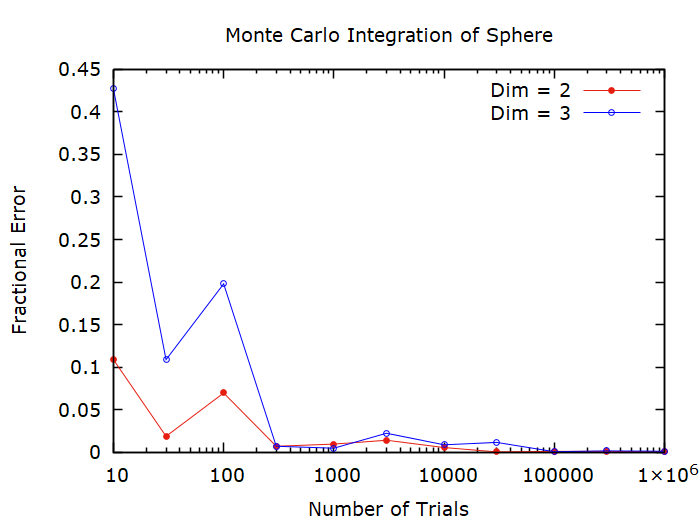
\includegraphics[scale=0.3]{dimverr.png}
  		\caption{Fractional error of the Monte Carlo integration of the 2D and 3D cases using the generalized program. While fluctuations are present early on, the error does decrease closer to 0 after 10000 trials. For this reason, we use 50000 trials for the determination of the values in Table \ref{tbl:1}.}
  		\label{gr:dimverr}
 	\end{center}
\end{figure}

\begin{table}[h] % table environment to enable captions and labels, [h] = 'here'
	\begin{center}
		\begin{tabular*}{\columnwidth}{| @{\extracolsep{\fill}} c c c c c | }
		\hline
Dim & Vcube & Vsphere & Vactual & FracErr \\
\hline\hline
$2$ & $4$ & $3.14$ & $3.142$ & $0.0004484$ \\ 
$3$ & $8$ & $4.192$ & $4.189$ & $0.0008465$ \\
$4$ & $16$ & $4.946$ & $4.935$ & $0.00237$ \\
$5$ & $32$ & $5.247$ & $5.264$ & $0.003194$ \\
$6$ & $64$ & $5.182$ & $5.168$ & $0.002731$ \\
$7$ & $128$ & $4.736$ & $4.725$ & $0.002432$ \\
$8$ & $256$ & $4.133$ & $4.059$ & $0.0184$ \\
$9$ & $512$ & $3.326$ & $3.299$ & $0.00832$ \\
$10$ & $1024$ & $2.515$ & $2.55$ & $0.01381$ \\
 		\hline
		\end{tabular*}
	\caption{Monte Carlo integration values of the unit hypersphere for dimensions 2 to 10. The number of trials for these values was 500000.} \label{tbl:1}
	\end{center}
\end{table}

\begin{figure}[htbp]
  	\begin{center}
 		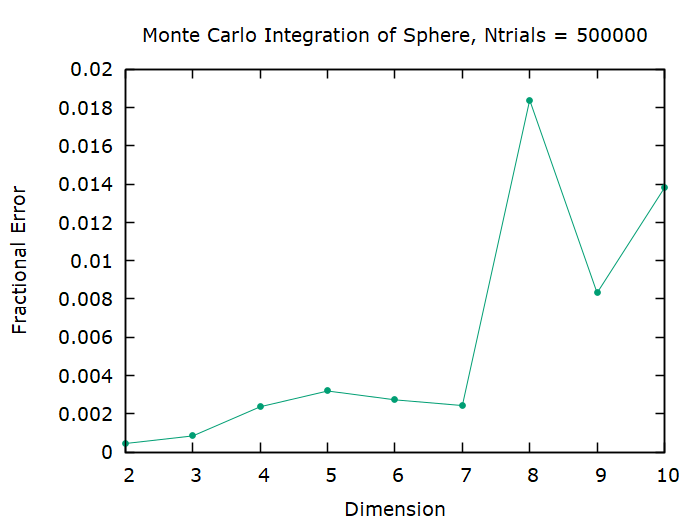
\includegraphics[scale=0.3]{errvdim.png}
  		\caption{The fractional error in Monte Carlo integration with varying dimension.}
  		\label{gr:errvdim}
 	\end{center}
\end{figure}

\begin{figure}[htbp]
  	\begin{center}
 		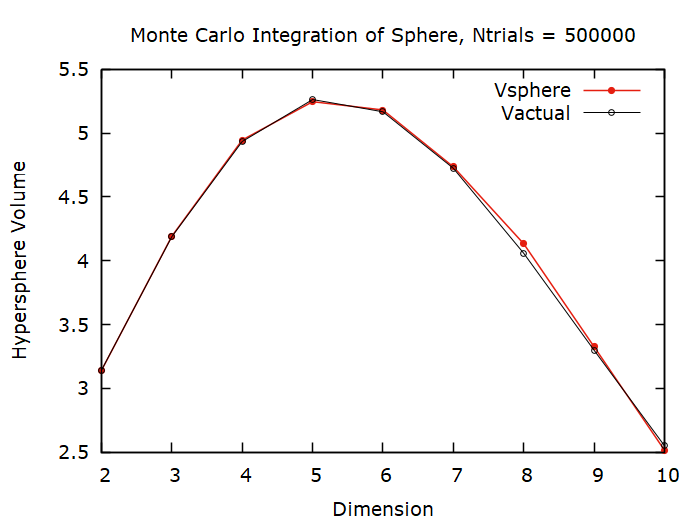
\includegraphics[scale=0.3]{volvdim.png}
  		\caption{Volume of the unit hypersphere in different dimensions. We can see clearly an odd fact that the volume has a peak at dimension 5, then decreases thereafter.}
  		\label{gr:volvdim}
 	\end{center}
\end{figure}

\section{Discussion and Analysis}
We are now able to analyze the behavior of the unit hypersphere through varying dimensions. It is evident from Figure \ref{gr:volvdim} that something strange happens when we reach dimension 5. The volume of the sphere actually begins to decrease, despite the volume of the cube containing it increasing. This can be inferred from Equation \ref{eqn:Vtrue} as well. As the degree of the cosine increases, the waves become sharper but still at amplitude 1. Thus the area under the curve for high powers of cosine are less than 1 and continually getting closer to 0. So at higher dimensions, the volume has factors that are decreasing it rather than increasing.
We can also see from Figure \ref{gr:errvdim} that the error is generally constant up until dimension 8. At that point, there is a significant jump in error. The height of the jump may be misrepresented here since the random nature of the calculation can cause fluctuations at such precise numbers. But there is a general increase by a factor of 10. So the relationship between the error and dimension isn't clear. I am not quite sure what causes this.

\section{Conclusions}
We were able to use Monte Carlo methods to find and analyze the volume of the unit hypersphere at dimensions higher than three. We found that the volume does not monotonically increase, but instead reaches a peak at dimension 5, then decreases towards 0 thereafter. Monte Carlo integration will be an important technique for other high dimension integration we may need to do in future problems. However, it seems we need an incredibly large number of trials to get an accurate value to fairly high precision. The random nature which causes such fluctuations in the error can be quite sensitive when looking at high precision. This implies that we must take caution in our values if we use Monte Carlo integration in that we can only expect a certain level of precision for very high numbers of trials. Nevertheless, it adds another tool in our repertoire for approximation in computational methods to solving physics problems. 

\section*{Acknowledgments}
\setlength{\parindent}{0cm}

\bibliographystyle{aipauth4-1}
\bibliography{bib5}



\end{document}